%# -*- coding: utf-8-unix -*-
%%==================================================

\chapter{疲劳检测经典算法和模型}

也许你听说过算法的5个特性:
\begin{enumerate}
    \item \textbf{输入}: 算法具有0个或多个输入
    \item \textbf{输出}: 算法至少有1个或多个输出
    \item \textbf{有穷性}: 算法在有限的步骤之后会自动结束而不会无限循环,并且每一个步骤可以在可接受的时间内完成
    \item \textbf{确定性}:算法中的每一步都有确定的含义,不会出现二义性
    \item \textbf{可行性}:算法的每一步都是可行的,也就是说每一步都能够执行有限的次数完成
\end{enumerate}

也许你曾听说过这几个公式:
\begin{align}
& \mbox{程序} = \mbox{算法} + \mbox{数据结构} \\
& \mbox{软件} = \mbox{程序} + \mbox{软件工程} \\
& \mbox{软件公司} = \mbox{软件} + \mbox{商业模式}
\end{align}

机器学习涉及到机器学习算法和模型的使用。对于初学者来说,这很容易让人混淆,因为“机器学习算法”经常与“机器学习模型”交替使用。这两个到底是一样的东西呢,还是不一样的东西?作为开发人员,你对排序算法、搜索算法等“算法”的直觉,将有助于你厘清这个困惑。因此在了解相应算法和模型之前,我们还是有必要先区分一下在机器学习中算法和模型\footnote{\url{https://blog.csdn.net/zandaoguang/article/details/107373743}}。

机器学习中的“算法”是在数据上运行以创建机器学习“模型”的过程。机器学习算法执行“模式识别”。算法从数据中“学习”,或者对数据集进行“拟合”。机器学习算法有很多。比如,我们有分类的算法,如 K- 近邻算法;回归的算法,如线性回归;聚类的算法,如 K- 均值算法。

机器学习中的“模型”是运行在数据上的机器学习算法的输出。模型表示机器学习算法所学到的内容。模型是在训练数据上运行机器学习算法后保存的“东西”,它表示用于进行预测所需的规则、数字和任何其他特定于算法的数据结构。

我举一些例子,可能会让人更清楚地明白这一点:
\begin{itemize}
    \item 线性回归算法的结果是一个由具有特定值的稀疏向量组成的模型。
    \item 决策树算法的结果是一个由具有特定值的 if-then 语句树组成的模型。
    \item 神经网络 / 反向传播 / 梯度下降算法一起产生一个由具有特定值的向量或权重矩阵和特定值的图结构组成的模型。
\end{itemize}

综上,我们可以得到两个公式:程序 = 算法 + 数据结构,模型 = 数据(结构) + 算法;这两个公式中,算法还是那个算法,而机器学习模型就好比软件工程中的程序了,但是它偏重于数学层面,而非应用层面。

\section{数据平衡算法}

常用的分类算法一般假设不同类的比例是均衡的,现实生活中经常遇到不平衡的数据集,比如广告点击预测(点击转化率一般都很小)、商品推荐(推荐的商品被购买的比例很低)、信用卡欺诈检测等等 \footnote{不平衡数据处理 \quad \url{https://mp.weixin.qq.com/s?__biz=MzAwMzIxMjIyMg==&mid=2651005812&idx=1&sn=b9819f04cb2ee9af21f4011d34013824&scene=0}}。

对于不平衡数据集,一般的分类算法都倾向于将样本划分到多数类,体现在模型整体的准确率很高。但对于极不均衡的分类问题,比如仅有1$\%$ 的人是坏人,99$\%$的人是好人,最简单的分类模型就是将所有人都划分为好人,模型都能得到99$\%$的准确率,显然这样的模型并没有提供任何的信息。在类别不平衡的情况下,对模型使用F值或者AUC值是更好的选择。

处理不平衡数据,可以从两方面考虑:

一是改变数据分布,从数据层面使得类别更为平衡;

二是改变分类算法,在传统分类算法的基础上对不同类别采取不同的加权方式,使得模型更看重少数类。

本小节对数据层面的一些方法做一个介绍,改变数据分布的方法主要是重采样:
\begin{itemize}
    \item 欠采样:减少多数类样本的数量
    \item 过采样:增加少数类样本的数量
    \item 综合采样:将过采样和欠采样结合
\end{itemize}

欠采样算法主要包括Nearmiss、Kmeans、TomekLinks和ENN,过采样算法主要包括SMOTE、ADASYN。

\subsection{基本概念}

这里要注意区分一下:过采样和欠采样是针对整个样本数据集来说的,目的是让数据集中样本类别保持平衡;而上采样和下采样是针对单个样本(信号,图片等)来说的,主要考虑在对样本的抽样上,怎样才能保证样本信息在采样过程中尽量不丢失部分重要信息,这里就要涉及到香农采样定理了\footnote{图像操作中的上采样、下采样,过采样、欠采样等 \quad \url{https://blog.csdn.net/qq_29566629/article/details/100183924}}。

\subsubsection{欠采样, 过采样}

针对一个数据集来说,重采样可以分为欠采样和过采样。

1、欠采样(undersampling)

减少多数类样本数量最简单的方法便是随机剔除多数类样本,可以事先设置多数类与少数类最终的数量比例ratio,在保留少数类样本不变的情况下,根据ratio随机选择多数类样本。

优点:操作简单,只依赖于样本分布,不依赖于任何距离信息,属于非启发式方法。

缺点:会丢失一部分多数类样本的信息,无法充分利用已有信息。\\ \\

2、过采样(Oversampling)

增加少数类样本数量最简单的方法便是随机复制少数类样本,可以事先设置多数类与少数类最终的数量比例ratio,在保留多数类样本不变的情况下,根据ratio 随机复制少数类样本。

在使用的过程中为了保证所有的少数类样本信息都会被包含,可以先完全复制一份全量的少数类样本,再随机复制少数类样本使得数量比例满足给定的ratio。

优点:操作简单,只依赖于样本分布,不依赖于任何距离信息,属于非启发式方法。

缺点:重复样本过多,容易造成分类器的过拟合。

\subsubsection{综合采样}

目前为止我们使用的重采样方法几乎都是只针对某一类样本:对多数类样本欠采样,对少数类样本过采样。也有人提出将欠采样和过采样综合的方法,解决样本类别分布不平衡和过拟合问题,本部分介绍其中的两个例子:SMOTE+Tomek links和SMOTE+ENN。

\footnote{\url{https://imbalanced-learn.org/stable/auto_examples/api/plot_sampling_strategy_usage.html#sphx-glr-auto-examples-api-plot-sampling-strategy-usage-py}}

\subsubsection{上采样,下采样}

针对一个样本, 重采样(重要性采样还是重新采样??)可分为上采样和下采样。这里以图片为例进行解释\footnote{图像操作中的上采样、下采样,过采样、欠采样等 \quad \ url{https://blog.csdn.net/qq_29566629/article/details/100183924}}

1、下采样(downsampling or subsampling)

缩小图像(或称为下采样(subsampled)或降采样(downsampled))的主要目的有两个:使得图像符合显示区域的大小;生成对应图像的缩略图。

2、上采样(upsampling)

图像放大几乎都是采用内插值方法,即在原有图像像素的基础上在像素点之间采用合适的插值算法插入新的元素。无论缩放图像(下采样)还是放大图像(上采样),采样方式有很多种。如最近邻插值,双线性插值,均值插值,中值插值等方法。在AlexNet中就使用了较合适的插值方法。各种插值方法都有各自的优缺点。


\subsection{SMOTE算法}

\subsection{TomekLinks算法}

\subsection{NearMiss算法}

\href{https://xueshu.baidu.com/usercenter/paper/show?paperid=28300870422e64fd0ac338860cd0010a&site=xueshu_se}{SMOTE: Synthetic Minority Over-sampling Technique}

\section{特征预处理}

\subsection{均值化}

\subsection{归一化}

\subsection{标准化}

\subsection{中心化}

\subsection{正则化}

\section{特征提取和特征选择}

特征提取和特征选择是数据降维的两种方法,这两者目的相同,但是却有所区别。特征提取是整合原始特征,可能会伴随着一些新的特征的产生,得到的新特征是原来特征的一个映射;特征选择是在保留原始特征上,去除无关紧要或庸余的特征。特征选择得到的特征是原来特征的一个子集。特征提取主要用于图像分析,信号处理和信息检索领域,在这些领域,模型精确度比模型可解释性要重要;特征选择主要用于数据挖掘,像文本挖掘,基因分析和传感器数据处理等\footnote{\url{https://blog.csdn.net/littlely_ll/article/details/71545929}} \footnote{\url{https://www.cnblogs.com/peizhe123/p/4713402.html}}。

\subsection{主成分分析(PCA)}

主成分分析(Principal Component Analysis,PCA),是一种统计方法。通过正交变换将一组可能存在相关性的变量转换为一组线性不相关的变量,转换后的这组变量叫主成分。它首先是由K. 皮尔森(Karl Pearson)对非随机变量引入的,尔后H.霍特林将此方法推广到随机向量的情形。信息的大小通常用离差平方和或方差来衡量。

\subsubsection{基本原理}

主成分分析是设法将原来众多具有一定相关性(比如P个指标),重新组合成一组新的互相无关的综合指标来代替原来的指标。

主成分分析,是考察多个变量间相关性一种多元统计方法,研究如何通过少数几个主成分来揭示多个变量间的内部结构,即从原始变量中导出少数几个主成分,使它们尽可能多地保留原始变量的信息,且彼此间互不相关.通常数学上的处理就是将原来P个指标作线性组合,作为新的综合指标。

最经典的做法就是用$F1$(选取的第一个线性组合,即第一个综合指标)的方差来表达,即$Var(F1)$越大,表示$F1$包含的信息越多。因此在所有的线性组合中选取的$F1$应该是方差最大的,故称$F1$为第一主成分。如果第一主成分不足以代表原来P个指标的信息,再考虑选取$F2$ 即选第二个线性组合,为了有效地反映原来信息,$F1$已有的信息就不需要再出现在F2 中,用数学语言表达就是要求$Cov(F1, F2)=0$,则称F2为第二主成分,依此类推可以构造出第三、第四,...,第P个主成分。

PCA有两种定义方式,第一种方式是把PCA定义为数据在低维线性空间上的正交投影,这个线性空间被称为主子空间(principal subspace),使得投影数据的方差最大化(Hotelling, 1933)。另一种方式则是将PCA定义为平均投影代价最小化的线性投影,平均投影代价是指数据点和它们的投影之间的平均平方距离(Pearson, 1901)。正交投影的过程如图\href{fig:3-1}{3-1}所示。

\begin{figure}[!htp]
\centering
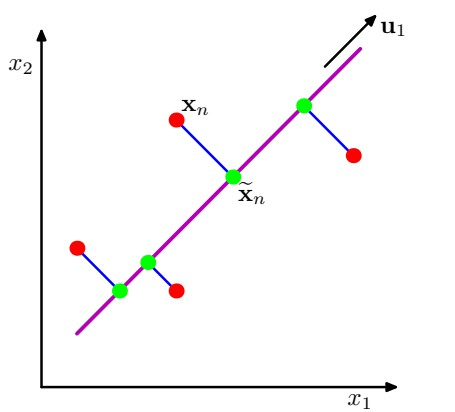
\includegraphics[width=3in]{example/pca1.jpg}
\caption{主成分分析寻找一个低维空间,被称为主子平面,用紫线表示,使得数据点(红点)在子空间上的正交投影能够最大化投影点(绿点)的方差。PCA 的另一个定义则是基于投影误差的平方和的最小值,用蓝线表示。}
\label{fig1:3-1}
\end{figure}

\subsubsection{算法步骤}

我们如何得到这些包含最大差异性的主成分方向呢?事实上,通过计算数据矩阵的协方差矩阵,然后得到协方差矩阵的特征值特征向量,选择特征值最大(即方差最大)的k个特征所对应的特征向量组成的矩阵。这样就可以将数据矩阵转换到新的空间当中,实现数据特征的降维。

已知$w_1, w_2, ... , w_m$是一组在新空间的维度为m下满足投影方差最大的基底。
$w_{m+1}$要满足的条件有:
\begin{enumerate}[label=\circled{\arabic*}]
    \item 模为1,$||w_{m+1}||= 1$;
    \item 与$w_1, w_2,..., w_m$都正交,$w^T_{m+1}w_j = 0$;
    \item $w^T_{m+1}X$的方差最大。
\end{enumerate}

在原始数据X(要去均值,也就是中心化)的协方差矩阵$\sum_X$ 做特征值分解(实对称矩阵一定能找到一个正交矩阵使其对角化,这个正交矩阵正是由其特征值对应的特征向量所组
成), 将特征值从大到小排序,其中最大的特征值$\lambda_1$ 所对应的特征向量$\omega_1$ 作用在样本X所得到的“新”特征$z^{(1)} = \omega_1^T X$ 称为第一主成分,随后是第二主成分$z^{(2)}$,第三主成分,..., 只保留k个主成分,构成样本$x_i$ 降维后的表示$z_i$, k的值可通过下式来确定:

\begin{eqnarray}
\frac{\sum_{i = 1}^k \lambda_i}{\sum_{j = 1}^d \lambda_j} \geq 85 \%
\end{eqnarray}

如果要从Z再重建到原先数据所在的空间中,需要做的变换是$WZ$。 最小均方重建误差的优化目标为:
\begin{align}
min_{W} ||X - WW^TX||^2 \\
st. \quad \quad W^TW = I
\end{align}
可以推导出,优化目标等价于
\begin{eqnarray}
max_W tr(W^T\sum_xW)
\end{eqnarray}


协方差矩阵的特征值特征向量有两种求解方法:特征值分解协方差矩阵、奇异值分解协方差矩阵,所以基本上PCA算法有两种实现方法:基于特征值分解协方差矩阵实现PCA算法、基于SVD 分解协方差矩阵实现PCA 算法\footnote{主成分分析(PCA)原理详解 \quad \url{https://blog.csdn.net/program_developer/article/details/80632779}}。

\begin{eqnarray}
F_p = a_{1i}*Z_{X1} + a_{2i}*Z_{X2} + .... + a_{pi}*Z_{Xp}
\end{eqnarray}

其中$a_{1i}, a_{2i}, ...,a_{pi}(i=1,...,m)$为X的协方差阵$\sum$ 的特征值所对应的特征向量,$Z_{X1}, Z_{X2}, ..., Z_{Xp}$ 是原始变量经过标准化处理的值,因为在实际应用中,往往存在指标的量纲不同,所以在计算之前须先消除量纲的影响,而将原始数据标准化(这里用的是Z 标准化)。

\begin{eqnarray}
A = (a_{ij})p \times m = (a_1,a_2,...,a_m), R_{ai} = \lambda_{i} \cdot a_{i}
\end{eqnarray}

R为相关系数矩阵,$\lambda_{i}$、$a_i$是相应的特征值和单位特征向量,$λ1 \geq λ2 \geq ...\geq λp \geq 0$。

进行主成分分析主要步骤如下:
\begin{figure}[!htp]
\centering
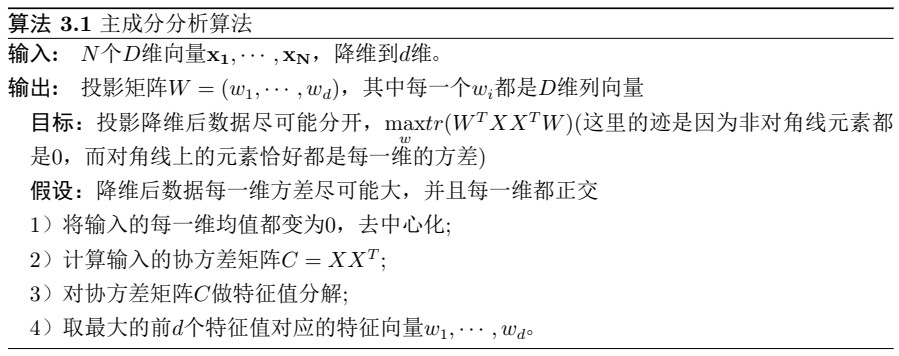
\includegraphics[width=5.5in]{example/pca.jpg}
\caption{PCA算法流程}
\label{fig1:3-1}
\end{figure}

假如经过PCA我们能得到降维后的三个成分,新特征$F$与原特征$f$ 变换关系表示为
\begin{align}
\begin{bmatrix}
F_1 \\
F_2 \\
F_3 \\
\end{bmatrix}
=
\begin{bmatrix}
a_{11} & a_{12} & a_{13} \\
a_{21} & a_{22} & a_{23} \\
a_{31} & a_{32} & a_{33} \\
\end{bmatrix}
\cdot
\begin{bmatrix}
f_1 \\
f_2 \\
f_3 \\
\end{bmatrix} \nonumber
\end{align}

常见的PCA还包括:最大方差形式的PCA,最小误差形式的PCA,最大似然PCA,核PCA等。

\subsubsection{作用}

1)主成分分析能降低所研究的数据空间的维数。即用研究m维的Y 空间代替p 维的X空间($m < p$),而低维的Y空间代替高维的x空间所损失的信息很少。即:使只有一个主成分Yl(即 m=1) 时,这个Yl 仍是使用全部X变量(p 个)得到的。例如要计算Yl的均值也得使用全部x的均值。在所选的前m 个主成分中,如果某个Xi的系数全部近似于零的话,就可以把这个Xi删除,这也是一种删除多余变量的方法。

2)有时可通过因子负荷$a_{ij}$的结论,弄清X变量间的某些关系。

3)多维数据的一种图形表示方法。我们知道当维数大于3时便不能画出几何图形,多元统计研究的问题大都多于3个变量。要把研究的问题用图形表示出来是不可能的。然而,经过主成分分析后,我们可以选取前两个主成分或其中某两个主成分,根据主成分的得分,画出n 个样品在二维平面上的分布况,由图形可直观地看出各样品在主分量中的地位,进而还可以对样本进行分类处理,可以由图形发现远离大多数样本点的离群点。

4)由主成分分析法构造回归模型。即把各主成分作为新自变量代替原来自变量x做回归分析。

5)用主成分分析筛选回归变量。回归变量的选择有着重的实际意义,为了使模型本身易于做结构分析、控制和预报,好从原始变量所构成的子集合中选择最佳变量,构成最佳变量集合。用主成分分析筛选变量,可以用较少的计算量来选择量,获得选择最佳变量子集合的效果。

\subsubsection{代码}

参考\href{https://github.com/heucoder/dimensionality_reduction_alo_codes}{主成分分析(PCA)源码}

\lstinputlisting[
    style       =   C,
    caption     =   {\bf PCA.py},
    label       =   {PCA.py}
]{./code/PCA.py}

\subsubsection{应用}

主成分分析是一种常用的多变量分析方法,被广泛应用于人口统计学、数量地理学、分子动力学模拟、数学建模、数理分析等学科,在区域经济发展评价,服装标准制定,满意度测评,模式识别,图像压缩等许多领域均有应用。

\subsection{因子分析(FA)}

因子分析(Factor Analysis) \footnote{因子分析(Factor Analysis)\quad \url{https://www.cnblogs.com/jerrylead/archive/2011/05/11/2043317.html}}

\subsection{独立成分分析(ICA)}


\subsection{线性判别分析(LDA)}

线性判别分析(LDA)是一种经典的有监督的线性学习方法,是一种判别模型,具有一定的预测功能,在二分类问题上最早由Fisher 在1936 年提出,亦称Fisher线性判别。线性判别的思想非常朴素:给定训练样例集,设法将样例投影到一条直线上,使得同类样例的投影点尽可能接近,异样样例的投影点尽可能远离;在对新样本进行分类时,将其投影到同样的直线上,再根据投影点的位置来确定新样本的类别。

\subsubsection{LDA的引出}

在经过特征提取以后,我们经常需要进行降维。首先我们简化一下问题便于阐述其原理:假设在二维特征空间中,有两类样本,那么我们的目标就是对给定的数据集,将其投影到一条直线上,但是投影的方法有千千万万种,那么我们该选择什么样的投影呢?如图\href{figure:3-3}{3-3}所示\footnote{Dimensionality Reduction——LDA线性判别分析原理篇 \quad \url{https://zhuanlan.zhihu.com/p/27899927?group_id=869893271453863936}}。

\begin{figure}[!htp]
\centering
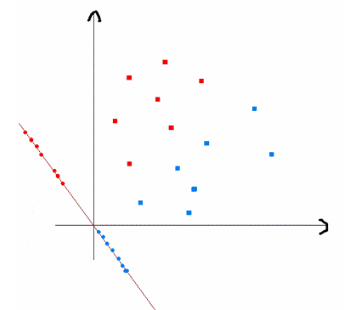
\includegraphics[width=3.5in]{example/LDA1.png}
\caption{利用投影进行特征降维}
\label{fig1:3-1}
\end{figure}

首先我们的任务是为了分类服务的,那么我们需要投影后的样本尽可能的分开,最简单的度量类别之间分开程度的方式就是类别均值投影之后的距离。

一种比较好的投影方式就是利用不同类别的数据的中心来代表这类样本在空间中的位置,考虑1个2分类问题。

给定特征为d维的N个样例,$x^{(i)} = \{ x_1^{(i)}, x_2^{(i)}, ... , x_d^{(i)}\}$,其中$N_1$个样例属于类别$\theta_1$,另外$N_2$个样例属于类别$\theta_2$,则两类的均值向量可以用下式计算得到。

\begin{eqnarray}
\mu_i = \frac{1}{N_i}\sum_{x \in \theta_i} x
\end{eqnarray}

同时保证让投影之后的中心距离尽可能的大,也就是:

\begin{eqnarray}
J(w) = |\tilde \mu_1 - \tilde \mu_2| = |w^T(\mu_1 - \mu_2)|
\end{eqnarray}

其中$\tilde \mu_i = \frac{1}{N_i}\sum_{y \in \theta_i} y = \frac{1}{N_i}\sum_{x \in \theta_i} w^T x = w^T \mu_i $ 是来自类别 $i$的投影数据的均值, $w^T$是我们的投影向量。但是,通过增大$w$,这个表达式可以任意增大。为了解决这个问题,我们可以将$w$限制为单位长度,即$\sum_i w_i^2 = 1$。

使用拉格朗日乘数法来进行有限制条件的最大化问题的求解,我们可以发现$ w \propto |\tilde \mu_2 - \tilde \mu_1|$。这个方法还有一个问题,如下图所示:

\begin{figure}[!htp]
\centering
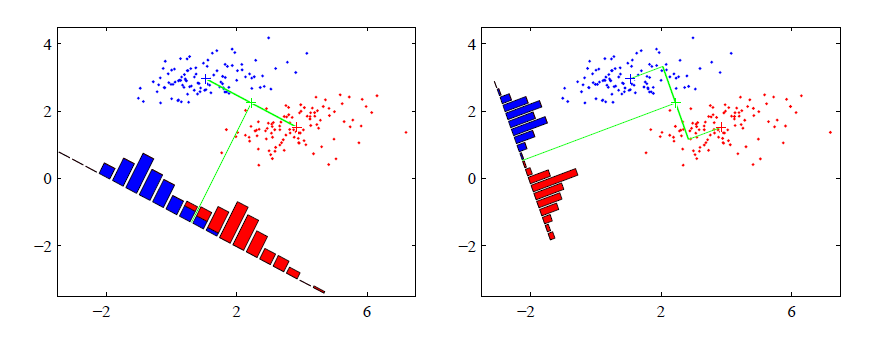
\includegraphics[width=5.5in]{example/LDA.png}
\caption{LDA的思想:最大化类间距离,最小化类内距离}
\label{fig1:3-1}
\end{figure}

左图为最大间隔度量的降维结果,这幅图中的两个类别在原始空维空间$(x1;x2)$中可以完美地被分开,但是当投影到连接它们的均值的直线上时,就有了一定程度的重叠。

换句话说,对于式\href{}{3-8},我们可能会直观理解,$J(w)$ 越大,两类样本的均值差距越大,对于两个类别的样本分离更明确。但如果只考虑$J(w)$ 是不行,如图\href{fig:3-5}{3-5} 所示:

样本点均匀分布在椭圆里,投影到横轴$x1$上时能够获得更大的中心点间距$J(w)$,但是由于有重叠,$x1$不能分离样本点。投影到纵轴$x2$ 上,虽然$J(w)$ 较小,但是能够分离样本点。因此我们还需要考虑样本点之间的方差,方差越大,样本点越难以分离,这一点我会在LDA推导中进行详细说明。

\begin{figure}[!htp]
\centering
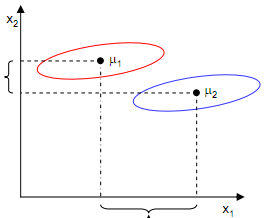
\includegraphics[width=3.5in]{example/LDA2.png}
\caption{两类均值向量$\mu_1,\mu_2$}
\label{fig1:3-1}
\end{figure}

因此,Fisher提出的思想:最大化一个函数,这个函数能够让类均值的投影分开得较大,同时让每个类别内部的方差较小,从而最小化了类别的重叠(右图中的结果)。

这也是LDA的中心思想即:最大化类间距离,最小化类内距离。

\subsubsection{LDA的推导}

这一小节会给出LDA的推导过程 \footnote{线性判别分析(Linear Discriminant Analysis)(一) \quad \url{https://www.cnblogs.com/jerrylead/archive/2011/04/21/2024384.html}},下式中没有提及到的数学符号请见上一小节:"LDA的引出"。

上一小节已经直观解释了单纯考虑$J(w)$会存在问题,因此需要使用另外一个度量值,称作散列值(scatter),对投影后的类求散列值,如下:

\begin{eqnarray}
\tilde s_i^2 = \sum_{y \in \theta_i}(y - \tilde \mu_i)^2
\end{eqnarray}

散列值的几何意义是样本点的密集程度,值越大,越分散,反之,越集中。

而我们想要的投影后的样本点的样子是:不同类别的样本点越分开越好,同类的越聚集越好,也就是均值差越大越好,散列值越小越好。正好,我们可以使用$J(w)$和S来度量,最终的度量公式(目标函数)是:

\begin{eqnarray}
J(w) = \frac{|\tilde u_1 - \tilde u_2|^2}{\tilde s_1^2 + \tilde s_2^2}
\end{eqnarray}

接下来的事就比较明显了,我们只需寻找使$J(w)$最大的$w$即可。

1)先处理分母,把类内散列值公式展开:

\begin{eqnarray}
\tilde s_i^2 = \sum_{y \in \theta_i}(y - \tilde \mu_i)^2 = \sum_{x \in \theta_i}(w^T x - w^T \mu_i)^2 = \sum_{x \in \theta_i} w^T(x - \mu_i)(x - \mu_i)^T w
\end{eqnarray}

我们可以定义$S_i = \sum_{x \in \theta_i}(x - \mu_i)(x - \mu_i)^T$,称其为散列矩阵。接着我们继续定义$S_w = S_1 + S_2$,其中$S_w$称为类内散列矩阵。

那么上式可以化简为:
\begin{align}
& \tilde s_i^2 = w^T S_i w \\
& \tilde s_1^2 + \tilde s_2^2 =  w^T S_w w
\end{align}

2)再处理分子,把类间散列值公式(均值方差公式)展开:
\begin{eqnarray}
(\tilde \mu_1 - \tilde \mu_2)^2 = (w^T\mu_1 - w^T\mu_2)^2 = w^T(\mu_1 - \mu_2)(\mu_1 - \mu_2)^T w = w^TS_Bw
\end{eqnarray}
其中$S_B$称为类间散列值,是两个向量的外积,虽然是个矩阵,但秩为1。

3)化简目标函数:
\begin{eqnarray}
J(w) = \frac{w^TS_B w}{w^TS_w w}
\end{eqnarray}

4)归一化$w$,变成带约束的优化问题

在我们求导之前,需要对分母进行归一化,因为不做归一的话,$w$ 扩大任何倍,都成立,我们就无法确定$w$。因此我们打算令$||w^TS_ww|| = 1$,那么加入拉格朗日乘子后,求导可得
\begin{align}
& c(w) = w^TS_Bw - \lambda(w^T S_Ww - 1)\\
& \Rightarrow \frac{dc}{dw} = 2S_Bw - 2\lambda S_W w = 0 \\
& \Rightarrow S_Bw = \lambda S_Ww
\end{align}

其中用到了矩阵微积分,求导时可以简单地把$w^TS_Ww$当做$S_Ww^2$ 看待。

如果$S_w$可逆,那么将求导后的结果两边都乘以$S_w^{-1}$,得到Fisher linear判别式:
\begin{eqnarray}
S_W^{-1} S_Bw = \lambda w
\end{eqnarray}

5)化简Fisher linear判别式:
\begin{eqnarray}
S_B = (\mu_1 - \mu_2)(\mu_1 - \mu_2)^T
S_B w = (\mu_1 - \mu_2)(\mu_1 - \mu_2)^Tw = (\mu_1 - \mu_2)* \lambda_w
\end{eqnarray}

代入上面的特征值公式,Fisher linear判别式可以化简成:
\begin{eqnarray}
S_W^{-1} S_B w = S_W^{-1} (\mu_1 - \mu_2)* \lambda_w = \lambda w
\end{eqnarray}

由于对$w$扩大缩小任何倍不影响结果,因此可以约去两边的未知常数$\lambda$和$\lambda_w$,得到:
\begin{eqnarray}
w = S_w^{-1}(\mu_1 - \mu_2)
\end{eqnarray}

至此,我们只需要求出原始样本的均值和方差就可以求出最佳的方向w,最终投影效果如下图所示。

\begin{figure}[!htp]
\centering
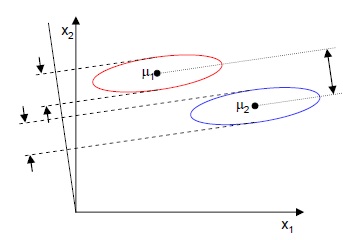
\includegraphics[width=3.5in]{example/LDA3.png}
\caption{Fisher Linear判别的最终投影效果}
\label{fig1:3-1}
\end{figure}

对于多类的线性判别分析(如图\href{figure:3-8}{3-8}所示),详细请见该博客《\href{https://www.cnblogs.com/jerrylead/archive/2011/04/21/2024384.html}{线性判别分析(Linear Discriminant Analysis)(一)}》

对于线性判别分析的使用说明,可参考该博客《\href{https://www.cnblogs.com/jerrylead/archive/2011/04/21/2024389.html}{线性判别分析(Linear Discriminant Analysis)(二)}》

\begin{figure}[!htp]
\centering
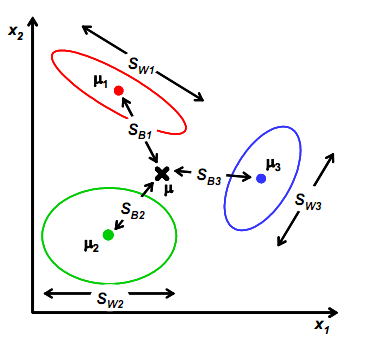
\includegraphics[width=3.5in]{example/LDA4.png}
\caption{对于多分类的LDA}
\label{fig1:3-8}
\end{figure}

\subsubsection{算法步骤}

LDA降维一般分为5个步骤(下式中没有提及到的数学符号请见上一小节:"LDA 的推导"):

1)计算数据集中每个类别样本的均值向量。

2)通过均值向量,计算类间散度矩阵$S_B$和类内散度矩阵$S_w$

3)对$S_W^{-1}S_B W=\lambda W$进行特征值求解,求出$S_W^{-1}S_B$ 的特征向量和特征值。

4)对特征向量按照特征值的大小降序排列,并选择前K个特征向量组成投影矩阵W。

5)通过D*K维的特征值矩阵将样本点投影到新的子空间中,Y=X*W。

\subsubsection{代码实现}

\lstinputlisting[
    style       =   C,
    caption     =   {\bf LDA.py},
    label       =   {LDA.py}
]{./code/LDA.py}

代码得改:w是投影矩阵,不单单是方向向量。

输出结果如图\href{figure:3-11}{3-11}所示。

\begin{figure}[!htp]
\centering
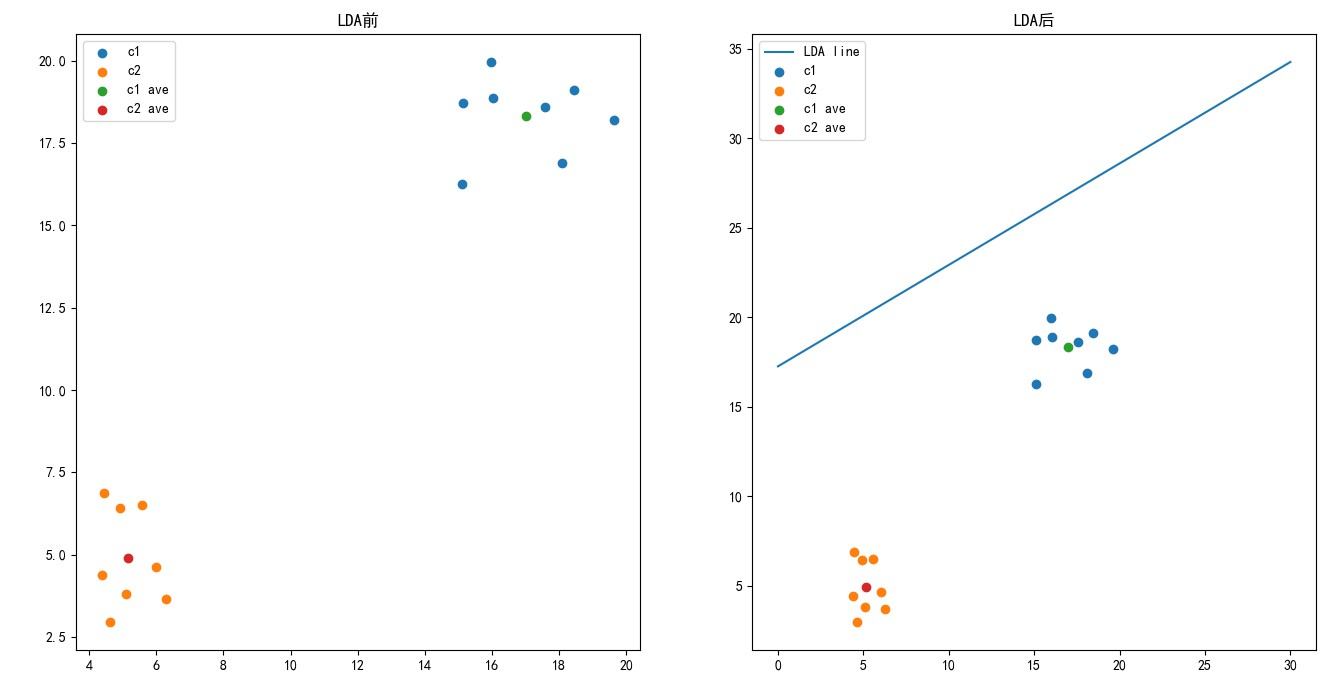
\includegraphics[width=4.5in]{example/LDA6.jpg}
\caption{LDA.py输出结果}
\label{fig1:3-8}
\end{figure}


\subsubsection{LDA和PCA的比较}

LDA和PCA的主要区别\footnote{用线性判别分析 LDA 降维 \quad \url{https://www.imooc.com/article/49321}}:

1)PCA属于无监督方法,数据没有标签时可以用它; 而LDA属于监督方法,考虑了数据的分类信息,这样数据在低维空间上就可以分类了,减少了很多的运算量, 如图\href{figure:3-9}{3-9}所示。
\begin{figure}[!htp]
\centering
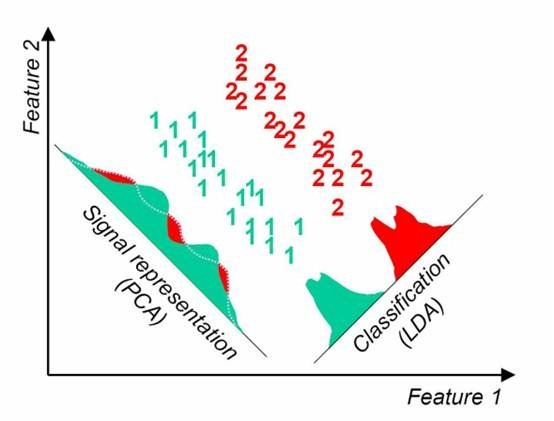
\includegraphics[width=3.5in]{example/PCAAndLDA.jpg}
\caption{PCA和LDA的降维比较}
\label{fig1:3-8}
\end{figure}

2)PCA主要是从特征的协方差角度考虑,追求的是在降维之后能够最大化保持数据的内在信息。它不考虑分类信息,因此,降低维度后,信息损失降到最低,但分类上可能会变得更加困难; 而LDA追求的是降维后的数据点尽可能容易被区分,降维后的样本数据在新的维度空间有最大的类间距离和最小的类内方差,数据在低维空间有最佳的可分离性。

3)PCA输出的维数和输入数据的维数是相关,原始数据是 n 维,那么PCA 后维度为 1、2 $\sim$ n 维; LDA 后的维数是和类别的个数相关的,原始数据是 n 维,一共有 C 个类别,那么 LDA 后维度为 1、2 $\sim$ C-1 维。

4)PCA投影的坐标系都是正交的;而LDA关注分类能力,不保证投影到的坐标系是正交的。

LDA与方差分析(ANOVA)和回归分析紧密相关,这两种分析方法也试图通过一些特征或测量值的线性组合来表示一个因变量。然而,方差分析使用类别自变量和连续因变量,而判别分析使用连续自变量和类别因变量(即类标签)。逻辑回归和概率回归比方差分析更类似于LDA,因为他们也是用连续自变量来解释类别因变量的。

\subsection{序列后向选择(SBS)}

序列后向选择( SBS , Sequential Backward Selection )

算法描述:从特征全集O开始,每次从特征集O中剔除一个特征x,使得剔除特征x后评价函数值达到最优。

算法评价:序列后向选择与序列前向选择正好相反,它的缺点是特征只能去除不能加入。

SBS属于贪心算法,容易陷入局部最优值\footnote{https://www.omegaxyz.com/2018/04/03/sfsandsbs/}。

\subsection{基于相关性的特征选择(CFS)}

论文地址:《\href{https://xueshu.baidu.com/usercenter/paper/show?paperid=111u0200ht6j0m202s2n0j40rm579580&site=xueshu_se&hitarticle=1}{Correlation-based Feature Selection for Discrete and Numeric Class Machine Learning}
》

\subsubsection{特征估计}

CFS估计特征子集并对特征子集而不是单个特征进行排秩,CFS的核心是采用启发的方式评估特征子集的价值,启发方式基于的假设是:好的特征子集包含与类高度相关的特征,但特征之间彼此不相关。

启发式方程如下:
\begin{align}
Merit_s = \frac{kr_{\overline{c}f}}{\sqrt{k+k(k-1)r_{\overline{f}f}}}
\end{align}

$Merit_s$为包含k个特征的特征自己$S$的启发式’merit’, $r_{\overline{c}f}$为特征-类平均相关性, $r_{\overline{f}f}$ 为特征-特征平均相关性。r为Pearson相关系数,所有的变量需要标准化。

CFS采用对称不确定性SU计算上式中的相关性

\begin{align}
SU =2.0 * [\frac{H(X) + H(Y) - H(X,Y)}{H(X) + H(Y)}]
\end{align}

启发式方法去除对类预测不起作用的特征变量,并识别与其他特征高度相关的特征。

\subsubsection{搜索特征子集空间}

CFS首先从训练集中计算特征-类和特征-特征相关矩阵,然后用最佳优先搜索(best first search)搜索特征子集空间。也可使用其他的搜索方法,包括前向选择(forward selection),后向消除(backward elimination)。前向选择刚开始没有特征,然后贪心地增加一个特征直到没有合适的特征加入。后向消除开始有全部特征,然后每一次贪心地去除一个特征直到估计值不再降低。最佳优先搜索和前两种搜索方法差不多。可以开始于空集或全集,以空集M 为例,开始时没有特征选择,并产生了所有可能的单个特征;计算特征的估计值(由merit值表示),并选择merit值最大的一个特征进入M,然后选择第二个拥有最大的merit 值的特征进入M,如果这两个特征的merit值小于原来的merit值,则去除这个第二个最大的merit值的特征,然后在进行下一个,这样依次递进,找出使merit 最大的特征组合。

它的时间复杂度为$m \times \frac{n^2 - n}{2}$,m是子集中特征个数,n是全部特征个数

\subsubsection{流程图}

CFS算法流程图如图\href{fig:3-15}{3-15}所示

\begin{figure}[!htp]
\centering
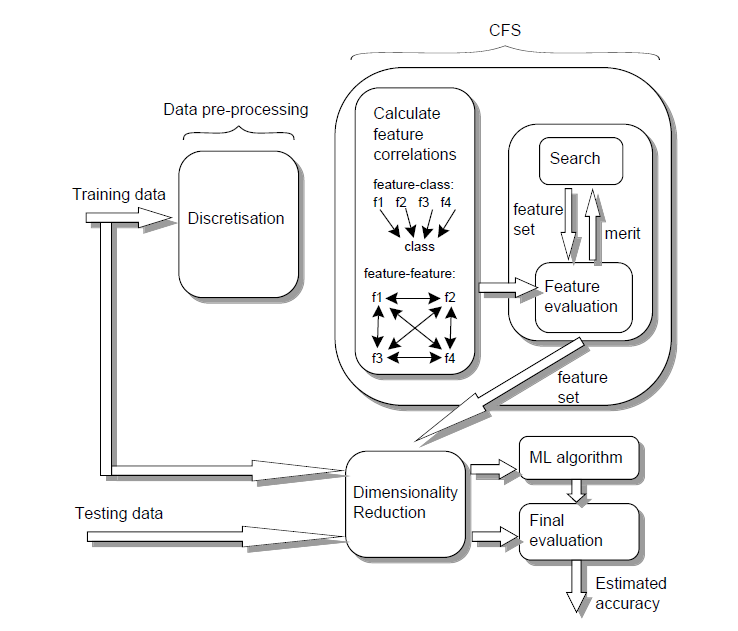
\includegraphics[width=5in]{example/CFS.png}
\caption{CFS算法流程图}
\label{fig1:3-15}
\end{figure}

\subsubsection{代码实现}

\lstinputlisting[
    style       =   C,
    caption     =   {\bf CFS.py},
    label       =   {CFS.py}
]{./code/CFS.py}

\subsection{信息增益算法(IG)}

%\begin{algorithm}[]
%\caption{:信息增益算法}
%\begin{algorithmic}[]
%\algorithmicrequire ~~ 训练数据集D和特征A \\

%\algorithmicensure ~~ 特征A对训练数据集D的信息增益g(D,A) \\

%\STATE (1) 计算数据集D的经验熵H(D) \\ $H(D) = - \sum_{k=1}^K \frac{|C_k|}{|D|}log_2\frac{|C_k|}{|D|}$
%\STATE

%\end{algorithmic}
%\end{algorithm}
%\renewcommand{\algorithmcfname}{算法}
\SetKw{KwInput}{\textbf{输入:}}{}
\SetKw{KwOutput}{\textbf{输出:}}{}
\begin{algorithm}[H]
\SetAlgoLined
\KwInput{训练数据集$D$和特征$A$} \\
\KwOutput{特征A对训练数据集$D$的信息增益$g(D,A)$ } \\
(1) 计算数据集D的经验熵$H(D)$ \\
\begin{array}{c}
\quad \quad H(D) = - \sum_{k=1}^{K} \frac{|C_k|}{|D|}log_2\frac{|C_k|}{|D|}
\end{array}

(2)计算特征A对数据集D的经验条件熵$H(D|A)$ \\
\begin{array}{c}
\quad \quad H(D|A)= \sum_{i=1}^{n} \frac{|D_i|}{|D|}H(D_i) = -\sum_{i=1}^n \frac{|D_i|}{|D|} \sum_{k=1}^K \frac{|D_{ik}|}{|D_i|}log_2\frac{|D_{ik}|}{|D_i|}
\end{array}

(3)计算信息增益 \\
\begin{array}{c}
\quad \quad g(D|A) = H(D) - H(D|A)
\end{array}
\caption{信息增益算法}
\end{algorithm}

\section{浅层分类器}

\subsection{支持向量机(SVM)}

\subsubsection{基本概念}

将数据进行分类是机器学习中的一项常见任务。假设某些给定的数据点各自属于两个类别,而目标是预测新数据点将在哪个类中。对于支持向量机,数据点被视为 $p$ 维向量,而我们想知道是否可以用 $p-1$ 维超平面来分开这些点,这就是所谓的线性分类器,有些时候可能存在多个超平面对数据进行分类。最佳超平面的一种合理选择是寻找以最大间隔把两个类分开的超平面。因此,我们要选择能够让矩离超平面最近的数据点和超平面的距离最大化的超平面。如果存在这样的超平面,则称为最大间隔超平面,而其定义的线性分类器被称为最大间隔分类器,这就是SVM的基本思想。

原始SVM算法是由弗拉基米尔·万普尼克和亚历克塞·泽范兰杰斯于1963 年发明的。1992年,Bernhard E. Boser、Isabelle M. Guyon 和弗拉基米尔·万普尼克提出了一种通过将核技巧应用于最大间隔超平面来创建非线性分类器的方法。1993年,Corinna Cortes和Vapnik 提出软间隔SVM,并于1995年发表。

\subsubsection{线性SVM}

已知测试集为:$\{(\overrightarrow{x_1},y_1),...,(\overrightarrow{x_n},y_n)\}$,其中$\overrightarrow{x_i}$ 是一个$p$维实向量,$y_i$ 是$x_i$ 的标签,取值为1 或者-1。

任何超平面都可以写成如下式子:
\begin{eqnarray}
\overrightarrow{w} \cdot \overrightarrow{x} - b = 0
\end{eqnarray}

其中$\overrightarrow{w}$(不必是归一化的)是该超平面的法向量。参数$\frac{b}{||\overrightarrow{w}||}}$决定着从原点沿法向量$\overrightarrow{w}$ 到超平面的偏移量。

1、硬间隔

如果这些训练数据是线性可分的,可以选择分离两类数据的两个平行超平面A,C,使得它们之间的距离尽可能大。在这两个超平面范围内的区域称为“间隔”,最大间隔超平面是位于它们正中间的超平面B。 这三个超平面可以由以下三个方程表示:
\begin{align}
& A: \quad \overrightarrow{w} \cdot \overrightarrow{x} - b = 1 \\
& B: \quad \overrightarrow{w} \cdot \overrightarrow{x} - b = 0 \\
& C: \quad \overrightarrow{w} \cdot \overrightarrow{x} - b = -1
\end{align}

A,C这两个超平面间的距离是$\frac{2}{||\overrightarrow{w}||}}$,如图\href{figure:3-12}{3-12} 所示。 因此要使两平面间的距离最大,我们需要最小化$||\overrightarrow{w}||$。 同时为了使得样本数据点都在A,C超平面以外,我们需要保证对于所有的$i$ 要满足以下条件:
\begin{align}
& \overrightarrow{w} \cdot \overrightarrow{x} - b \geq 1, \mbox{若}y_i = 1\\
& \overrightarrow{w} \cdot \overrightarrow{x} - b \leq -1,\mbox{若}y_i = -1
\end{align}
这些约束表明每个数据点都必须位于间隔的正确一侧。这两个式子可以整合成一个式子:
\begin{align}
& y_i (\overrightarrow{w} \cdot \overrightarrow{x} - b) \geq 1, for \quad all 1 \leq i \leq n
\end{align}

这样就变成了一个带约束的优化问题
\begin{align}
& ojective \quad function. \quad \min ||\overrightarrow{w}|| \\
& st. \quad \quad y_i (\overrightarrow{w} \cdot \overrightarrow{x} - b) \geq 1, \quad  for \quad all \quad 1 \leq i \leq n
\end{align}

\begin{figure}[!htp]
\centering
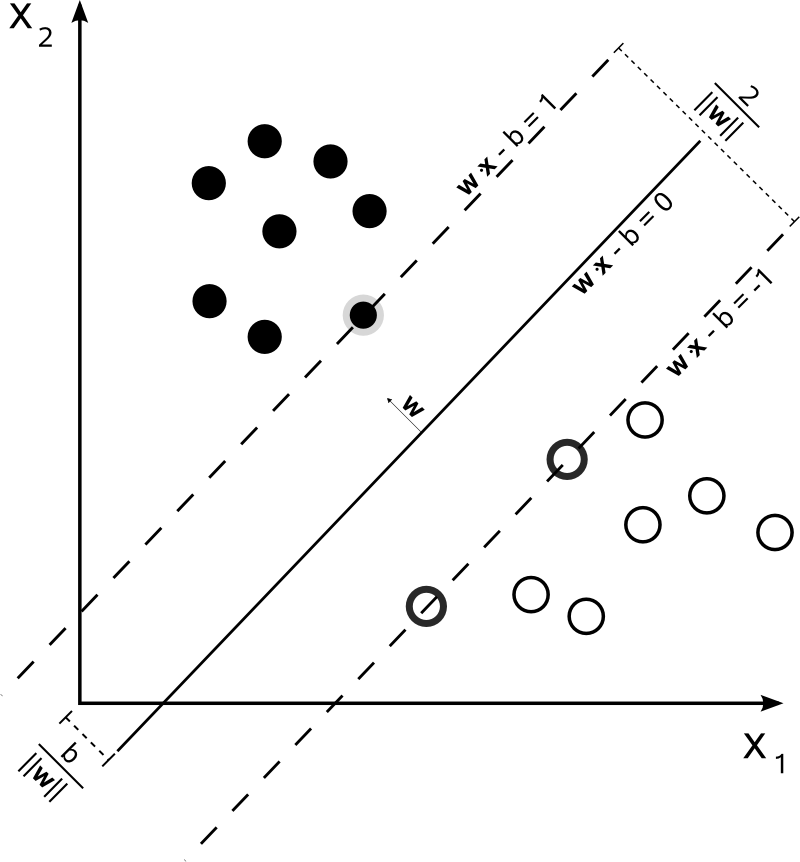
\includegraphics[width=3.5in]{example/SVM.png}
\caption{SVM最大间隔超平面}
\label{fig1:3-8}
\end{figure}

这个问题的解$\overrightarrow{w}$与$b$决定了最终的分类器$\overrightarrow{x} \mapsto sgn(\overrightarrow{w} \cdot \overrightarrow{x} - b)$,最大间隔超平面完全是由最靠近它的那些$\overrightarrow{x_i}$确定的。这些$\ overrightarrow{x_i}$ 叫做支持向量。

2、软间隔
为了将SVM扩展到数据线性不可分的情况,我们引入铰链损失函数:
\begin{align}
max(0,1 - y_i (\overrightarrow{w} \cdot \overrightarrow{x} - b))
\end{align}

当约束条件满足时,即
\begin{align}
& y_i (\overrightarrow{w} \cdot \overrightarrow{x} - b) \geq 1, \quad for \quad all \quad 1 \leq i \leq n
\end{align}

也就是如果$\overrightarrow{x_i}$位于边距的正确一侧时,此函数为零。对于间隔的错误一侧的数据,该函数的值与距间隔的距离成正比。 然后我们希望最小化如下式子:
\begin{align}
[\frac{1}{n} \sum_{i=1}^n max(0,1 - y_i (\overrightarrow{w} \cdot \overrightarrow{x} - b))] + \lambda||\overrightarrow{w}||^2
\end{align}

其中参数$\lambda$用来权衡增加间隔大小与确保$\overrightarrow{x_i}$位于间隔正确一侧之间的关系。因此,对于足够小的$\lambda$值,如果输入数据是可以线性分类的,则软间隔SVM与硬间隔SVM将表现相同,但即使不可线性分类,仍能学习出可行的分类规则。

\subsubsection{非线性分类}

万普尼克在1963年提出的原始最大间隔超平面算法构造了一个线性分类器。而1992年,Bernhard E. Boser、Isabelle M. Guyon和弗拉基米尔·万普尼克提出了一种通过将核技巧(最初由Aizerman et al.提出)应用于最大边界超平面来创建非线性分类器的方法。所得到的算法形式上类似,除了把点积换成了非线性核函数。这就允许算法在变换后的特征空间中拟合最大间隔超平面。该变换可以是非线性的,而变换空间是高维的;虽然分类器是变换后的特征空间中的超平面,但它在原始输入空间中可以是非线性的。

值得注意的是,更高维的特征空间增加了支持向量机的泛化误差,但给定足够多的样本,算法仍能表现良好。

常见的核函数包括:
\begin{itemize}
    \item 齐次多项式:
        \begin{align}
            k(\overrightarrow{x_i},\overrightarrow{x_i}) = (\overrightarrow{x_i},\overrightarrow{x_j})^d
        \end{align}
    \item 非齐次多项式:
         \begin{align}
            k(\overrightarrow{x_i},\overrightarrow{x_j}) = (\overrightarrow{x_i},\overrightarrow{x_j} + 1)^d
        \end{align}
    \item 高斯径向基函数:
        \begin{align}
            k(\overrightarrow{x_i},\overrightarrow{x_j}) = exp(-\gamma ||\overrightarrow{x_i} - \overrightarrow{x_j}||^2)
        \end{align}
        其中$\gamma > 0$,有时参数化表示为$\gamma = \frac{1}{2\sigma^2}$
    \item 双曲正切:
         \begin{align}
            k(\overrightarrow{x_i},\overrightarrow{x_j}) = tanh(-\kappa \overrightarrow{x_i} \cdot \overrightarrow{x_j} + c)
        \end{align}
        其中一些(而非所有)$\kappa > 0$且$c<0$
\end{itemize}

由等式$k(\overrightarrow{x_i},\overrightarrow{x_j}) = \varphi(\overrightarrow{x_i}) \cdot \varphi(\overrightarrow{x_j})$,核函数与$\varphi(\overrightarrow{x_i})$有关。变换空间中也有$w$值,
$\overrightarrow{w} = \sum_i \alpha_i y_i \varphi(\overrightarrow{x_i})$。与$w$的点积也要用核技巧来计算,即$\overrightarrow{w} \cdot \varphi(\overrightarrow{x}) = \sum_i \alpha_i y_i k(\overrightarrow{x_i},\overrightarrow{x})$。

\subsubsection{代码实现}

\lstinputlisting[
    style       =   C,
    caption     =   {\bf SVM.py},
    label       =   {SVM.py}
]{./code/SVM.py}


\subsubsection{应用}

用于文本和超文本的分类,图像分类,图像分割,蛋白质分类等

\subsection{提升树(Adaboost)}

\subsection{随机森林(Random Forest)}

\section{深度学习模型}

\subsection{深度置信网络(DBN)}

\subsection{隐马尔可夫模型(HMM)}

\subsection{循环神经网络(RNN)}

\subsection{长短期记忆网络(LSTM)}

\section{模型评估}

\subsection{分类和回归}

分类和回归的区别在于输出变量的类型\footnote{分类和回归的区别 \quad \url{https://blog.csdn.net/rocling/article/details/89010773}}。 定量输出称为回归,或者说是连续变量预测;定性输出称为分类,或者说是离散变量预测。

输入变量与输出变量均为变量序列的预测问题为标注问题

举个例子:
预测明天的气温是多少度,这是一个回归任务;
预测明天是阴、晴还是雨,就是一个分类任务。

分类模型和回归模型本质一样,分类模型是将回归模型的输出离散化。

举几个例子:

1. Logistic Regression 和 Linear Regression:

\begin{itemize}
    \item Linear Regression: 输出一个标量 $wx+b$,这个值是连续值,所以可以用来处理回归问题。
    \item Logistic Regression:把上面的 $wx+b$ 通过sigmoid函数映射到$(0,1)$ 上,并划分一个阈值,大于阈值的分为一类,小于等于分为另一类,可以用来处理二分类问题。更进一步:对于N分类问题,则是先得到N组w值不同的 $wx+b$,然后归一化,比如用softmax函数,最后变成N个类上的概率,可以处理多分类问题。 \\
\end{itemize}

2. Support Vector Regression 和 Support Vector Machine:

\begin{itemize}
    \item SVR:输出$wx+b$,即某个样本点到分类面的距离,是连续值,所以是回归模型。
    \item SVM:把这个距离用 $sign(\cdot)$ 函数作用,距离为正(在超平面一侧)的样本点是一类,为负的是另一类,所以是分类模型。\\
\end{itemize}

3. 神经网络用于分类和回归:

\begin{itemize}
    \item 用于回归:最后一层有m个神经元,每个神经元输出一个标量,m个神经元的输出可以看做向量 v,现全部连到一个神经元上,则这个神经元输出$wv+b$,是一个连续值,可以处理回归问题,跟上面 Linear Regression 思想一样。
    \item 用于N分类:现在这m个神经元最后连接到 N 个神经元,就有 N 组$w$值不同的$wv+b$,同理可以归一化(比如用softmax)变成 N个类上的概率。
\end{itemize}

分类模型和回归模型的评估指标如表\href{table:3-1}{3-1},\href{table:3-2}{3-2}所示\footnote{\url{https://my.oschina.net/u/4013614/blog/2437427}}。

\begin{table}[]
\centering
\caption{分类模型评估指标}
\label{table:3-1}
\begin{tabular}{|l|l|}
\hline
\textbf{指标}          & \textbf{描述}    \\ \hline
Precision            & 精确度            \\ \hline
Recall               & 召回率            \\ \hline
F1                   & F1值            \\ \hline
Confusion Matrix     & 混淆矩阵           \\ \hline
ROC                  & ROC曲线          \\ \hline
AUC                  & ROC曲线下的面积      \\ \hline
\end{tabular}
\end{table}

\begin{table}[]
\caption{回归模型评估指标}
\label{table:3-2}
\centering
\begin{tabular}{|l|l|}
\hline
\textbf{指标}                 & \textbf{描述} \\ \hline
Mean Square Error(MSE,RMSE) & 平均方差        \\ \hline
Absolute Error(MAE,RAE)     & 绝对误差        \\ \hline
R-Squared                   & R平方值        \\ \hline
\end{tabular}
\end{table}

\subsection{混淆矩阵(Confusion matrix)}

\subsubsection{二分类的混淆矩阵}

什么是TP,TN,FP,FN?其实就是对两种类别(0,1),以及这两种类别对应的两种预测结果(0,1)进行编码,得到4种结果。

FP表示实际为负但被预测为正的样本数量,TN表示实际为负被预测为负的样本的数量,TP表示实际为正被预测为正的样本数量,FN表示实际为正但被预测为负的样本的数量。这几个变量可以用表\href{table:3-3}{3-3}的混淆矩阵表示。这里要注意的是,FP,TP,TN,FN是针对预测结果而言的,第一个字母表示预测是否正确,第二个字母表示预测类别。

\begin{table}[]
\caption{二分类混淆矩阵}
\label{table:3-3}
\centering
\begin{tabular}{|l|l|l|l|}
\hline
\multicolumn{2}{|l|}{\multirow{2}{*}{\textbf{Confusion Matrix}}} & \multicolumn{2}{l|}{真实值} \\ \cline{3-4}
\multicolumn{2}{|l|}{}    & P  & N  \\ \hline
\multirow{2}{*}{预测值} & P' & TP & FP \\ \cline{2-4}
                     & N' & FN & TN \\ \hline
\end{tabular}
\end{table}

混淆矩阵的每一列(行)代表了预测类别,每一列(行)的总数表示预测为该类别的数据的数目;每一行(列)代表了数据的真实归属类别,每一行(列)的数据总数表示该类别的数据实例的数目。

\subsubsection{多分类的混淆矩阵}

\begin{figure}[!htp]
\centering
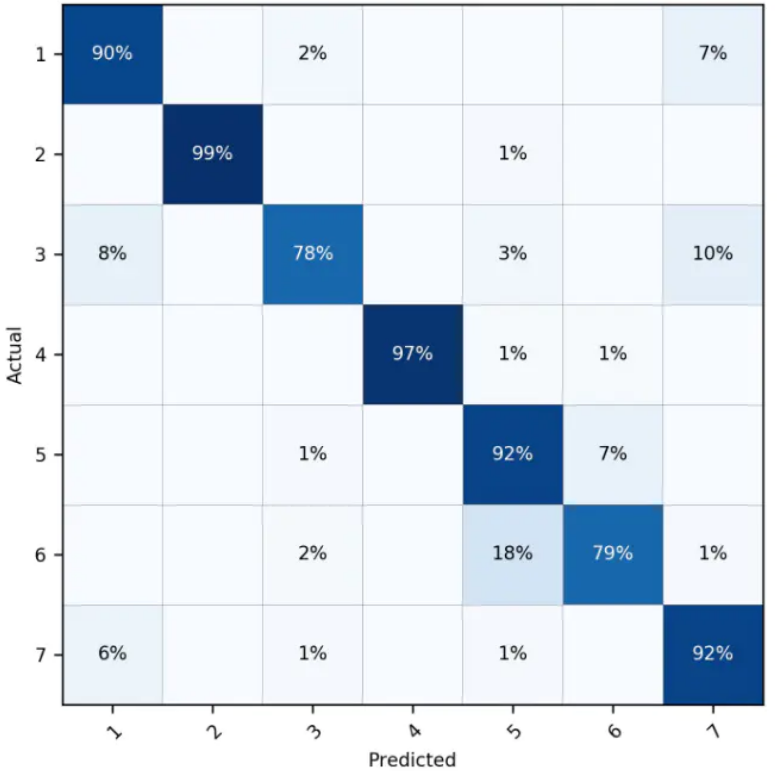
\includegraphics[width=4.5in]{example/ConfusionMatrix1.png}
\caption{多分类的归一化的混淆矩阵}
\label{fig1:3-15}
\end{figure}

参考资料\footnote{\url{https://en.wikipedia.org/wiki/Confusion_matrix}} \footnote{\url{https://www.jianshu.com/p/cd59aed787cf}}

\subsubsection{混淆矩阵的作用}

1、第一个是混淆矩阵能够帮助我们迅速可视化各种类别误分为其它类别的比重,这样能够帮我们调整后续模型,比如一些类别设置权重衰减\footnote{\url{https://zhuanlan.zhihu.com/p/46204175}}!

2、在一些论文的实验分析中,可以列出混淆矩阵,行和列均为label种类,可以通过该矩阵验证自己model预测复杂label的能力强于其他model,只要自己model复杂label误判为其它类别比其他model误判的少,就可以说明自己model预测复杂label的能力强于其他model。

\subsection{Precision,Recall,Accuracy,F1}

\subsubsection{精确率}

精确率是针对我们预测结果而言的,它表示的是预测为正的样本中有多少是真正的正样本。那么预测为正就有两种可能了,一种就是把正类预测为正类(TP),另一种就是把负类预测为正类(FP)。精确率计算公式如下\footnote{\url{https://www.zhihu.com/question/19645541/answer/91694636}}
\begin{align}
& Precision = \frac{TP}{TP + FP}
\end{align}

以目标检测为例,正类是指目标的类别,即前景(1,2,3,4..),而负类为背景(0),我们在计算精确率时只需考虑预测的结果是否为正类即可。假设我们想求第i类物体的检测精确率,我们需要在最终预测的第i类物体中,找到正确划分的(TP)和非正确划分的(FP)。

还是有点难理解?以二分类的人脸检测为例,人脸类别为1,其他背景类别为0,假设一张图片中共有6张人脸,并且经过模型的学习,最终输出长度为8的人脸位置序列,非人脸位置序列构成背景位置序列。经过与原图片标注序列的比对,统计人脸预测正确的数目为TP,预测错误的数目为FP,$TP + FP = 8$,根据公式就能计算了。

用通俗的话来讲,就是:你认为的该类样本,有多少是猜对了。

你也许会有疑问,对于多分类的目标检测,TP,FP要如何计算呢?其实我们可以将第i类定义为正类(前景),把其他类定义为负类(背景),把多分类的TP,FP计算问题转换成而分类的TP,FP计算问题。

\subsubsection{召回率}

召回率是针对我们原来的样本而言的,它表示的是样本中的正例有多少被预测正确了。那也有两种可能,一种是把原来的正类预测成正类(TP),另一种就是把原来的正类预测为负类(FN)。召回率计算公式如下。
\begin{align}
& Recall = \frac{TP}{TP + FN}
\end{align}

还是以人脸检测为例,假设一张图片中共有6张人脸,并且经过模型的学习,最终输出一系列人脸位置序列,非人脸位置序列构成背景位置序列。这两个序列与原图片标注序列比对后,我们可以计算人脸预测正确的数目TP,背景错误预测的数目FN,$TP + FN = 6$,根据公式就能计算出召回率了。

用通俗的话来讲,就是:该类样本有多少被找出来了。

\subsubsection{准确率}

准确率需要全面考虑预测结果的正确性,这个预测结果既包括正类,也包括负类。还是以人脸检测为例,假设一张图片中共有6张人脸,并且经过模型的学习,最终输出长度为8的人脸位置序列,非人脸位置序列构成背景位置序列。对于一张图片,$TP + FN = 6$,$TP + FP = 8$,$TN$是正确检测背景的数目,这样$TP+FN+FP+TN$包含原图片中所有的人脸,以及被检测到的背景图片。

\begin{align}
& Accuracy = \frac{TP+TN}{TP+FN+FP+TN}
\end{align}

\subsubsection{F1-Score}

F1 score 是对精度和召回率的调和平均\footnote{\url{https://www.jianshu.com/p/1afbda3a04ab}}:
\begin{align}
& F1 = 2 * \frac{Precision * Recall}{Precision + Recall}
\end{align}

我们使用调和平均而不是简单的算术平均的原因是:调和平均可以惩罚极端情况。一个具有 1.0 的精度,而召回率为 0 的分类器,这两个指标的算术平均是 0.5,但是 $F1$ score 会是 0。$F1$ score 给了精度和召回率相同的权重,它是通用 $F\beta$指标的一个特殊情况,在 $F\beta$中,$\beta$可以用来给召回率和精度更多或者更少的权重。(还有其他方式可以结合精度和召回率,例如二者的几何平均,但是 F1 score 是最常用的。) 如果我们想创建一个具有最佳的精度—召回率平衡的模型,那么就要尝试将 F1 score 最大化。

\subsection{ROC曲线}

\subsubsection{TPR,FPR}

ROC曲线是Receiver Operating Characteristic Curve的简称,中文名为“受试者工作特征曲线”\footnote{sklearn ROC曲线使用 \quad \ url{https://blog.csdn.net/hfutdog/article/details/88079934}}。

要绘制ROC曲线,我们需要先了解横坐标假阳性率(False Positive Rate,FPR)和纵坐标真阳性率(True Positive Rate,TPR)是如何计算的(不要和Precision,Recall弄混了)。
\begin{align}
& FPR = \frac{FP}{FP + TN} \\
& TPR = \frac{TP}{TP + FN}
\end{align}

从混淆矩阵也可以看到$N = FP+TN$是实际为负的样本数量,$T = TP+FN$是实际为正的样本数量,因此,FPR,TPR公式为:
\begin{align}
& FPR = \frac{FP}{N} \\
& TPR = \frac{TP}{T}
\end{align}

图\href{fig1:3-17}{3-17}是一个ROC曲线,现在我们对其进行分析。
\begin{figure}[!htp]
\centering
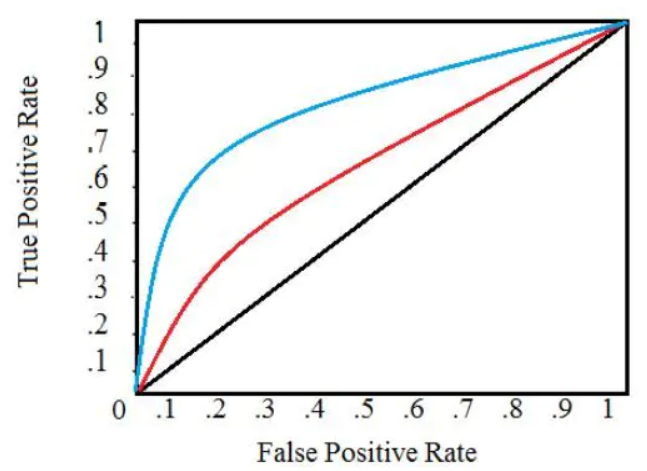
\includegraphics[width=4in]{example/ROC.png}
\caption{多模型的ROC曲线}
\label{fig1:3-15}
\end{figure}

黑色对角线表示随机分类器,红色和蓝色曲线表示两种不同的分类模型。对于给定的模型,只能对应一条曲线。但是我们可以通过调整对正例进行分类的阈值来沿着曲线移动。通常,当降低阈值时,会沿着曲线向右和向上移动。

在阈值为 1.0 的情况下,我们将位于图的左下方,因为没有将任何数据点识别为正例,这导致没有真正例,也没有假正例(TPR = FPR = 0)。当降低阈值时,我们将更多的数据点识别为正例,导致更多的真正例,但也有更多的假正例 (TPR 和 FPR 增加)。最终,在阈值 0.0 处,我们将所有数据点识别为正,并发现位于 ROC 曲线的右上角 ( TPR = FPR = 1.0 )。

最后,我们可以通过计算曲线下面积 ( AUC ) 来量化模型的 ROC 曲线,这是一个介于 0 和 1 之间的度量,数值越大,表示分类性能越好。在上图中,蓝色曲线的 AUC 将大于红色曲线的 AUC,这意味着蓝色模型在实现准确度和召回率的权衡方面更好。随机分类器 (黑线) 实现 0.5 的 AUC。

\subsubsection{ROC曲线绘制和分析}

接下来我们看看ROC曲线究竟是如何绘制的\footnote{牢记分类指标:准确率、精确率、召回率、F1 score以及ROC \url{https://www.jianshu.com/p/1afbda3a04ab}}。

举个例子,假设我们的任务是为 100 名病人诊断一种在普通人群中患病率是 50$\%$ 的疾病。假设有一个模型,我们输入关于患者的信息,并得到 0 到 1 之间的分数。我们可以改变将患者标记为正例 (有疾病) 的阈值,以最大化分类器性能。我们将以 0.1 为增量从 0.0 到 1.0 评估阈值,在每个步骤中计算 ROC 曲线上的精度、召回率、F1 score 以及在 ROC 曲线上的位置。通过设置阈值,我们可以计算TPR,FPR,如表\href{tab:3-4}{3-4}所示。
\begin{table}[!htp]
\centering
\caption{模型在每个阈值下的结果}
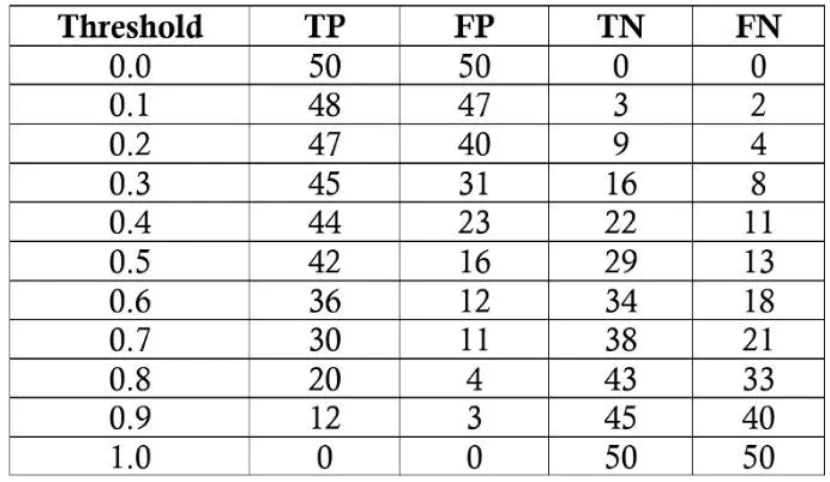
\includegraphics[width=4.5in]{example/ROC2.png}
\label{fig1:3-15}
\end{table}

接着我们可以绘制出ROC曲线,如图\href{fig1:3-17}{3-17}所示。
\begin{table}[!htp]
\centering
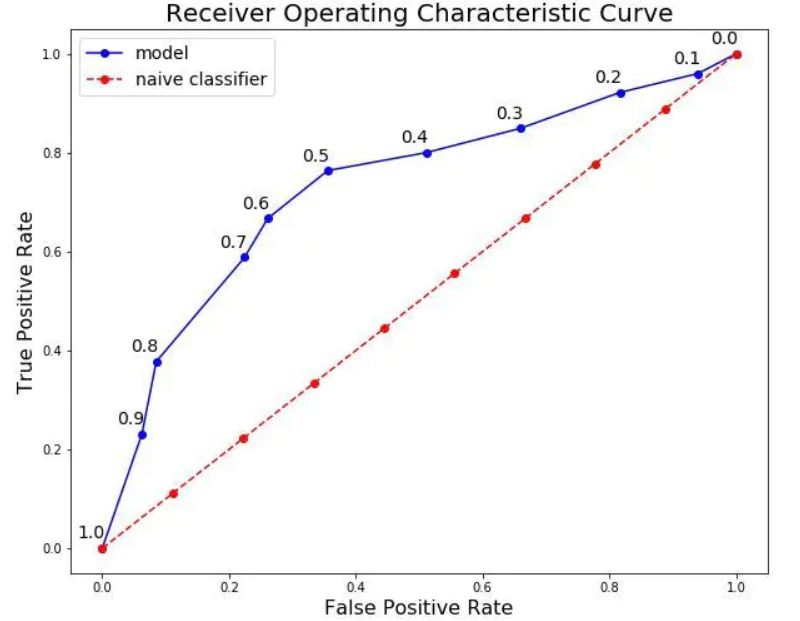
\includegraphics[width=4.5in]{example/ROC3.png}
\caption{ROC曲线绘制}
\label{fig1:3-17}
\end{table}

在阈值等于1.0的点,我们将任何病人归类为正常人,因此模型的召回率和精度都是0。随着阈值的减小,召回率增加了,因为我们发现更多的患者患有该疾病(患病为正类,正常为负类)。然而,随着召回率的增加,精度会降低,因为除了增加真正例(TP)之外,还会增加假正例(TP)。在阈值为 0.0 的时候,我们的召回率是完美的——我们发现所有的患者都患有这种疾病——但是精度很低,因为有很多假正例。通过更改阈值并选择最大化 F1 score 的阈值,最终我们可以得到在不同阈值下Precision,Recall,TPR,FPR,F1-Score的结果。

\begin{table}[!htp]
\centering
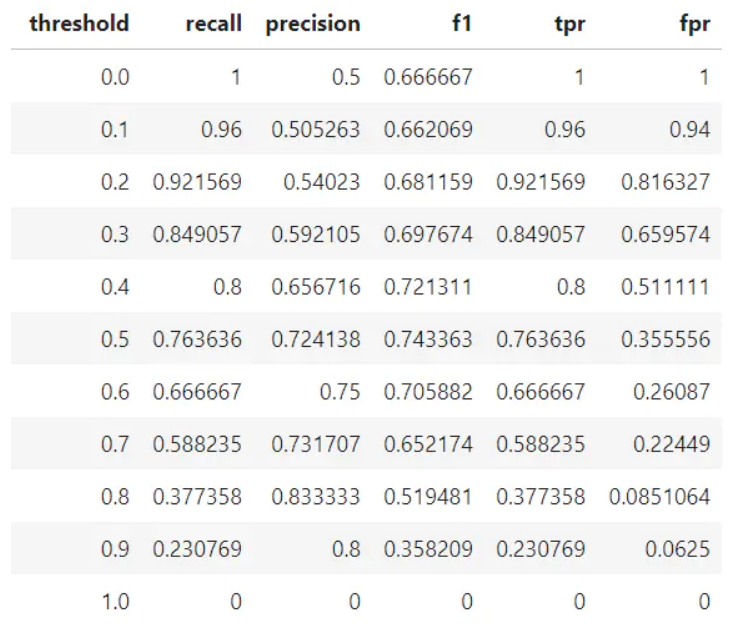
\includegraphics[width=4.5in]{example/ROC4.png}
\caption{在不同阈值下相关指标的取值}
\label{fig1:3-17}
\end{table}

基于 F1 score,整体最佳的模型出现在阈值为 0.5 的地方。如果我们想要在更大程度上强调精度或者召回率,我们可以选择这些指标上最佳时对应的模型。

\subsection{Kappa}

